\section{Experimental Methods}
\subsection{Photon Beam}
% ToDo: Think about if/where to include the calculation of the ratio of knockout neutrons to fission neutrons. Have only done calculation for Thorium.
A bremsstrahlung photon beam is produced passing 10.5 MeV electrons through a 1" thick slab of aluminum.
Aluminum was chosen as the radiator because it has a neutron knockout threshold above the energy of the electron beam.
This ensured that the bremsstrahlung radiator would not be a source of fast neutrons which would have the potential to make their way into the experimental cell and cause false neutron events.
Downstream from the bremsstrahlung radiator, a sweeping magnet removes excess electrons from the photon beam (see Figure~\ref{fig:Facility}).
After the sweeping magnet, the beam travels through a series of polyethylene and lead collimators.
Figure~\ref{fig:BremDist} shows the energy distribution of photons that reach the target according to MCNP simulation that included the creation and collimation of the bremsstrahlung photons.

\begin{figure}[h]
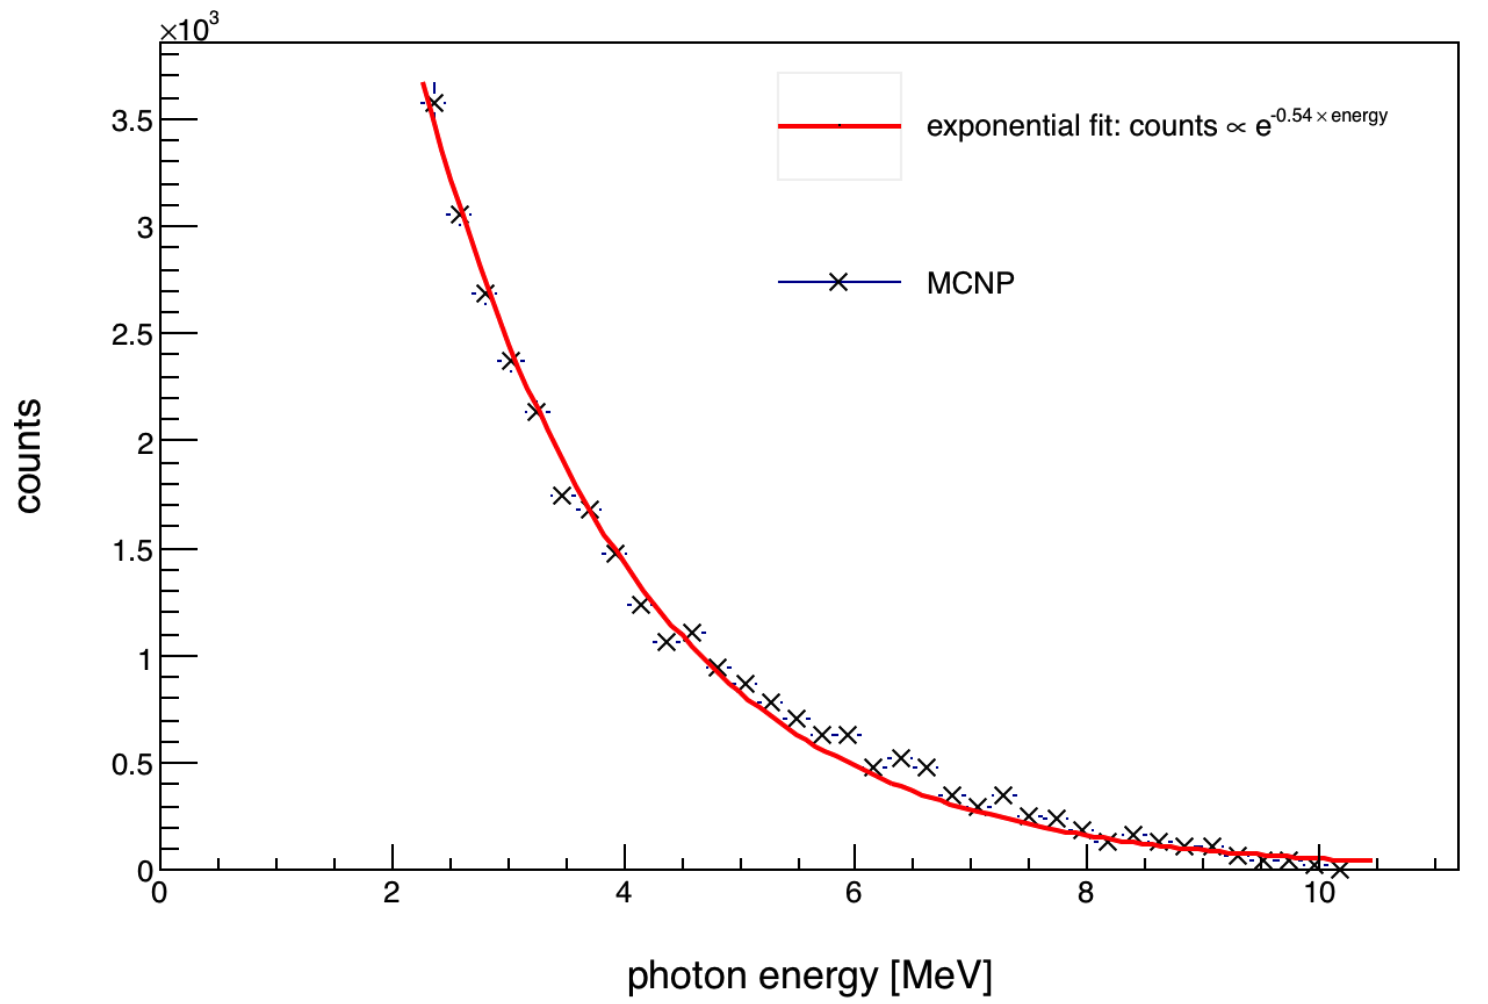
\includegraphics[width=0.9\textwidth]{Content/Methods/MCNPBremDistribution.png}
\caption{MCNP simulation of the energy distribution of the photons that reach the target.
The points are from the simulation.
The line is an exponential fit of the form $Ae^{-bx}$.}
\label{fig:BremDist}
\end{figure}

Thr reason for choosing a beam energy of 10.5 is that when attempting a measurement of prompt neutrons from photofission, an ambiguity can arise between neutrons from photofission and neutrons from $(\gamma, xn)$ if $x$ is greater than two.
The two reactions have similar cross-sections within the GDR region, and there is significant overlap between the energy spectra of the neutrons.
Because the current measurement is concerned only with observing two neutrons in coincidence, it suffices to set the Bremsstrahlung end-point below the target's ($\gamma, 2n$) threshold, which is $\sim$12 MeV for $^{238}U$.
Setting the end-point below the ($\gamma, 2n$) threshold does not eliminate the possibility of detecting two neutrons from  two ($\gamma, 1n$) reactions in a single pulse, which is referred to as an accidental coincidence.
An \textit{accidental} neutron coincidence occurs when two uncorrelated neutrons are detected in the same pulse.
The rate of accidentals follow the poissonian distribution, setting them apart from correlated events, and as a result, accidentals can be subtracted from the data.
The details and justifications for this procedure are discussed in section~\ref{Subtraction of Accidentals}.

The electron beam pulse width was set to 3 ns and had a 1.1A peak current, with a repetition rate of 240 Hz.
The 3 ns pulse width is not a large source of error in the measurements of neutron time of flight (ToF), since neutron events had a median TOF of $\approx$80 ns.
ToF is the time taken for a particle to travel from the target to the face of a detector.
The accelerator's current was set by requiring that there be, on average, fewer than one fission per pulse in order to diminish the number of accidentals.
% ToDo Discussion about the LINAC's low duty factor??

\subsection{Particle time of flight determination}
\label{reconstruction}
Each of the scintillators were equipped with two PMTs, one fixed at each end of the scintillator, with the exception of those located farthest downstream at $\pm30^{\circ}$ which each had a single PMT (see Figure~\ref{fig:DetGeom}).
In order to diminish dead-time, the detectors at $\pm30^{\circ}$ were segmented to create two independent detectors.
See section~ref{section:Detectors} for a more detailed discussion about the detectors at $\pm30^{\circ}$.
A ten cm block of a non-scintillating material was fixed between each PMT and the scintillator.
This backs the PMTs off from the scintillator so that light produced near the ends have a good line of sight to the PMT.
The timing resolution of each PMT is $\sim$2.5ns, however, the main source of uncertainly in the time of a particle hit is the variation in the time taken for scintillation light to propagate to the PMTs.
The time of events in the PMTs was always taken relative to a signal provided by the accelerator at the beginning of each pulse, referred to as the \textit{beam gun}.

ToF was used to distinguish between photons and neutrons, and to measure neutron energy.
Scintillation light that is detected by the PMTs has a measured effective index of refraction of $\sim$3.
Consequently, there can be up to an 8 ns delay between when a particle scintillates in the detector and the scintillation light reaches a PMT.
The effective index of refraction is found by measuring the time taken for scintillation light to travel the full length of the detector.
The actual index of refraction of the material is about half that value, a difference which is the result of light rays bouncing from the walls of the scintillator on their way to a PMT.
The time of flight was calculated by taking the average between the times of signals in the top and bottom PMTs, and then subtracting a calibration offset.
In taking the average, there is a reduction in the sensitivity of the result to the variation of propagation times as a function of the position at which the particle scintillated.
This cannot be done in the detectors located at $\pm30^{\circ}$, because they have only one PMT.
However, since they are 1/3 the length of the rest, scintillation light takes at most only 2.5 ns to propagate to the PMT, which is a tolerable amount of random error.
See section~\ref{Errors} for a deeper discussion of experimental errors.

The ToF of a particle obeys the following relationship:
\begin{displaymath}
\text{ToF}_i = t_{i}^0 + \Delta t_{\text{avg}}
\end{displaymath}
where $\text{ToF}_i$ is the ToF of a particle observed in detector $i$, $t_{i}^0$ is a constant timing offset, which is the same for every pulse, and $\Delta t_{\text{avg}} $ is the average between the timing of signals in the top and bottom PMTs of a given scintillator.
The reason for the subscript, $i$, is that the timing offset is different for each scintillator due to, for example, differences in the lengths of the PMT signal cables.
Any process that produces a timing delay that does not change from pulse to pulse contributes to $ t_{i}^0$.
Examples of this are:
\begin{itemize}
\item the time required for photons to travel from the bremsstrahlung radiator to the target
\item the propagation of signals through the wires connecting the PMTs
\item delays in the electronics
\item the transit time in the PMTs.
\item the time required for scintillation light to propagate from the point of creation to both PMTs.
\end{itemize}
The final example above is nearly constant only after the average between two PMTs is taken, $\Delta t_{\text{avg}}$, at which point this effect produces standard deviation of 3 ns in measured ToF.
The time required for scintillation light to travel to a single PMT can vary from $\approx$1 ns for particles that scintillate near a PMT, to $\approx$10 ns for particles that scintillate at the opposing end of the scintillator.
Variance in ToF measurements due to this is reduced by taking the average between the timing of signals from both PMTs of a scintillator.
$\Delta t_{\text{avg}}$ is 1/2 times the sum of the two times, and this sum includes the time for light to travel to both PMTs, which is just the time for light to travel the total length of the detector.
This value is a constant if the scintillation light travels parallel to the detector's length.
This isn't always the case, however, so the effective velocity at which scintillation light travels lengthwise through the detector has non-zero variance which contributes to the uncertainty of ToF measurement.
The setup favors the detection of scintillation photons that travel lengthwise through the scintillator, since these travel the shortest distance and therefore experience less attenuation.
In taking the average between two PMTs, the uncertainty in ToF is reduced by about a factor of three compared to using a single PMT.

\begin{figure}[h]
\includegraphics[width=0.7\textwidth]{Content/Methods/LightPaths.png}
\caption{The average of times taken for scintillation light to travel from the point of its creation to each PMT has low variance.
This average includes the time required for light to travel the full length of the detector, which is a constant for photons that travel exactly parallel to the length of the detector.
Scintillation photons that travel parallel to the length of the detector are favored for detection by the PMTs because they reach the PMT first and experience less attenuation.
Therefore, the distribution of $\Delta t_{\text{avg}}$ is reflective of the ToF distribution of the particle's producing scintillation light.}
\label{fig:LightPaths}
\end{figure}

The variance of the effective velocity of scintillation light was measured using a $^{60}$Co source, which emits coincident photons.
The $^{60}$Co source is placed at several positions along the face of a lead shielded scintillator.
At each position, a small hole is drilled through the lead to give the $^{60}$Co source a line-of-sight to a well defined point on the scintillator.
A high timing-resolution photon detector is placed next to the $^{60}$Co source.
When the $^{60}$Co source decays, emitting two photons simultaneously, one photon is detected by the high timing-resolution detector serving as the ``start'' time, and the other photon scintillates in the detector being calibrated.
The times of signals from each PMT, taken relative to the start trigger, are averaged.
The photons from $^{60}$Co cause scintillation at a specified location, so variation remaining in the result is due to varying paths taken by the scintillation light, and is a reflection of the error in ToF measurement.
These results can be seen in figures~\ref{fig:Co60Validation} and~\ref{fig:Co60ValidationProject}.
% **ToDo: Make a figure for the setup of the co60 calibration.
\begin{figure}[]
    \centering
    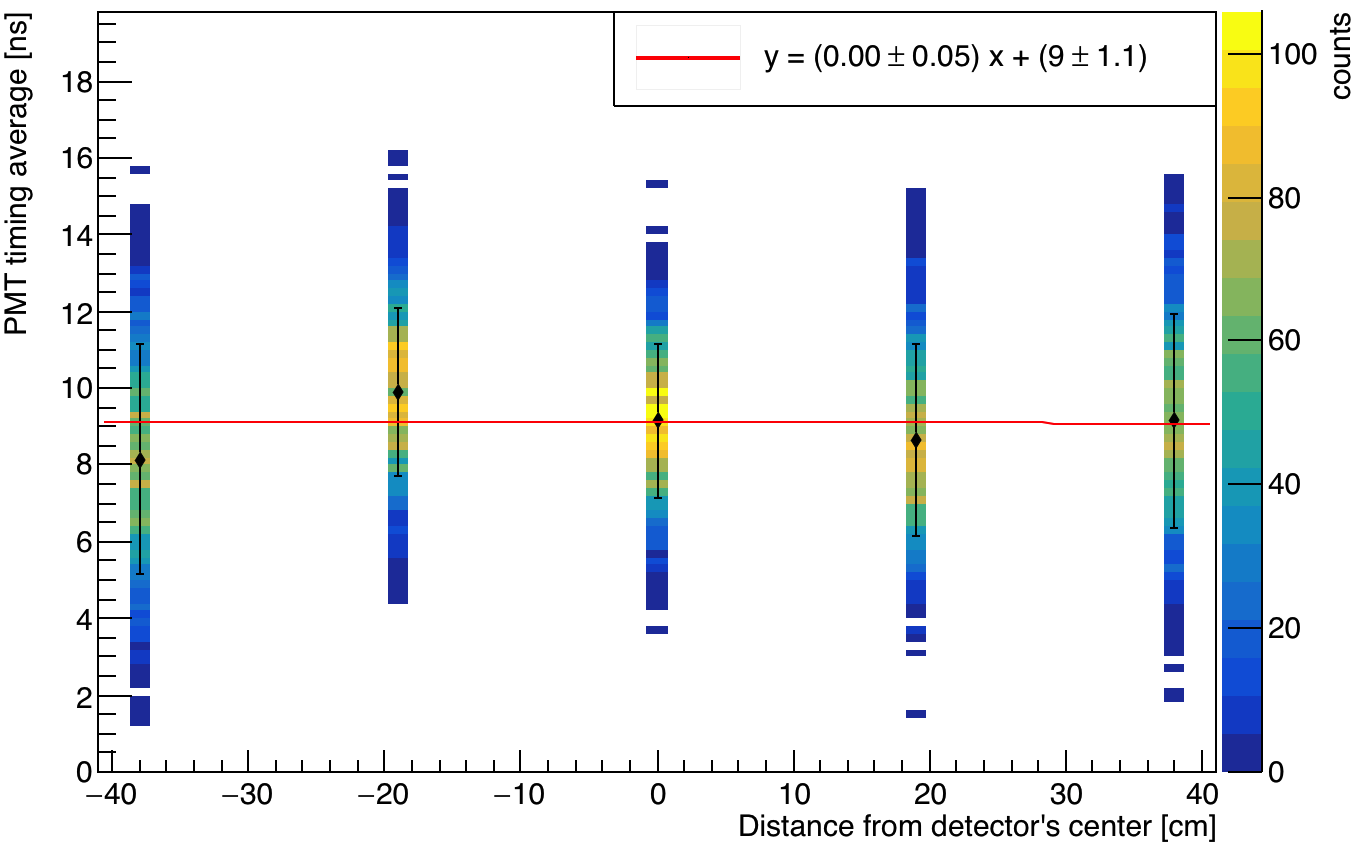
\includegraphics[width = 0.9\textwidth]{Content/Methods/CO60Validation.png}
    \caption{A $^{60}$Co source, which emits coincident photons, is placed at several positions along the face of a lead shielded scintillator.
    At each position, a small hole is drilled through the lead to give the $^{60}$Co source a line-of-sight to a well-defined point on the scintillator.
    Then, a high timing resolution scintillation photon detector made from ATP plastic is placed close to the $^{60}$Co source.
    When the $^{60}$Co source decays, emitting two photons simultaneously, one photon is detected by the high timing-resolution detector serving as the ``start'' time, and the other scintillates in the detector being calibrated.}
    \label{fig:Co60Validation}
\end{figure}
\begin{figure}
    \centering
    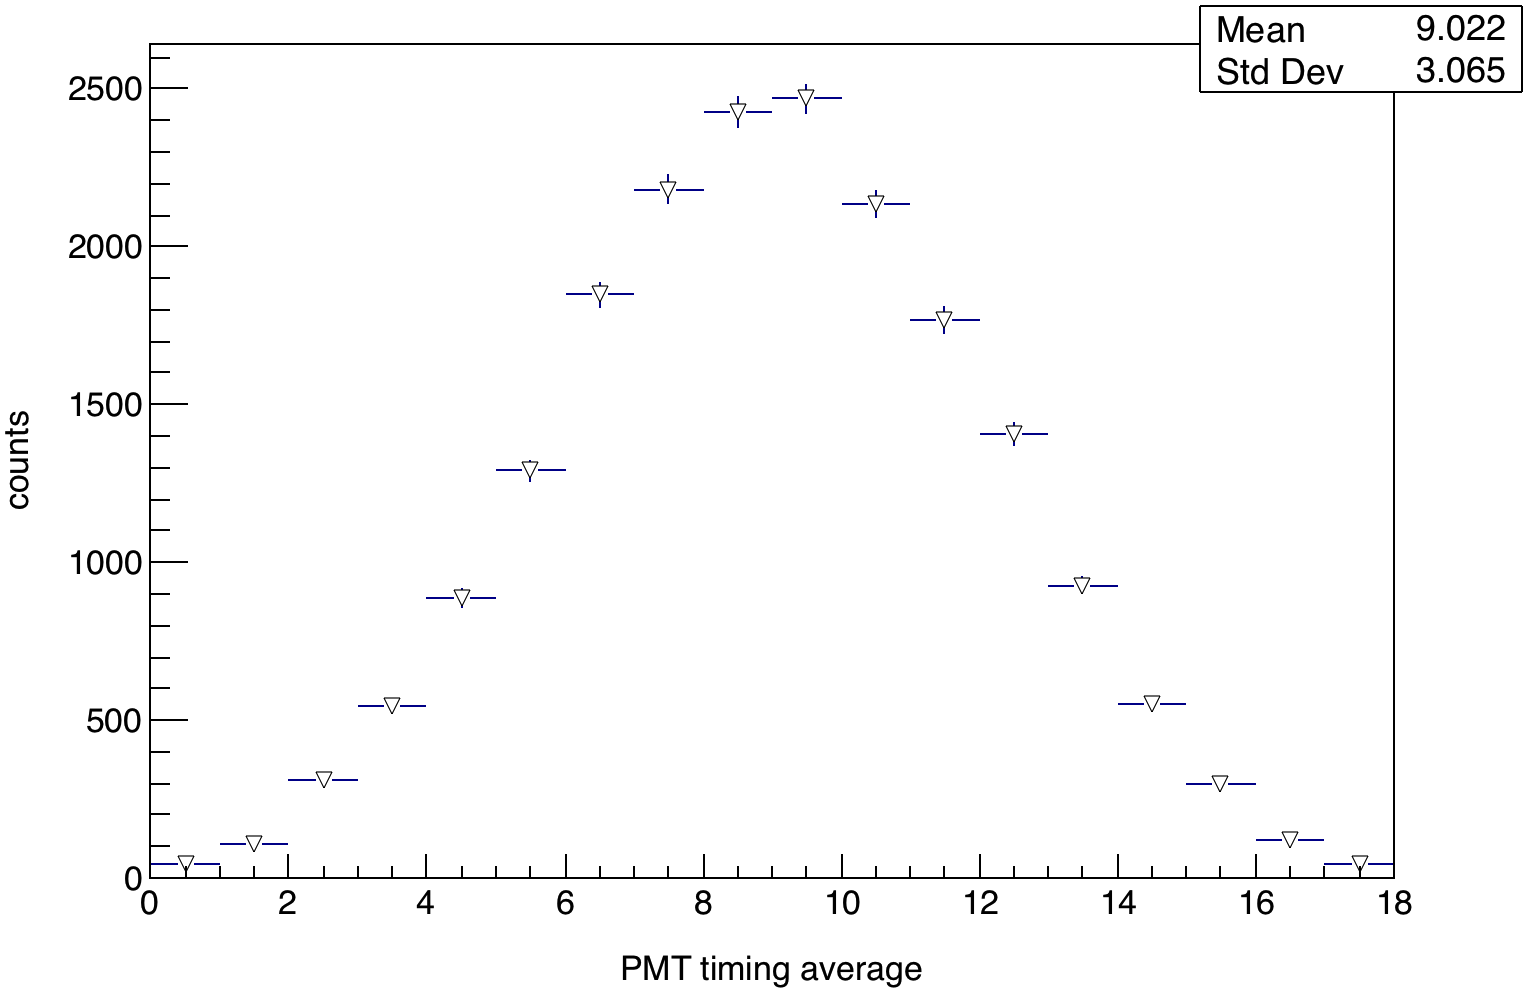
\includegraphics[width = 0.9\textwidth]{Content/Methods/CO60ValidationProject.png}
    \caption{
    The sum of times in the top and bottom PMTs are reflective of the time taken from scintillation light to travel the full length of the scintillator.
    Taken during calibration with a $^{60}$Co source.
    Ideally, the time taken for scintillation light to travel the length of the detector would be a constant, and the ToF resolution would be equal to the resolution of the PMTs at $\approx$ 1 ns.
    This is not the case, however, because scintillation light doesn't always take the shortest path to a PMT.
    The 3 ns standard deviation of this curve represents the uncertainty in the time at which a particle is detected.
    This plot is the result of projecting the data used in fig~\ref{fig:Co60Validation} onto the y-axis.
}
    \label{fig:Co60ValidationProject}
\end{figure}

The value of the constant offset for ToF calculation is determined by observing photons that scattered from the target.
Comparing the timing spectra of a non-neutron producing target made from aluminum, to the spectra produced when no target is used reveals a prominent peak caused by the scattering of photons from the target.
Aluminium does not produce photo-neutrons because the beams's Bremsstrahlung end-point is below Aluminium's ($\gamma$, n) threshold.
Photons scattered from the target must travel between 125 cm to 130 cm to reach a face of a detector, depending on whether the photons reach the detector near the center or at the edge.
It takes light 4.0 ns and 4.3 ns to travel 125 cm and 130 cm, respectively.
The difference between these two times is negligible for these purposes, so the ToF of photons that scatter from the target is assumed to be 4 ns.
With this assumption, the location of the photon peak in the timing spectra can be used to calculate the offset in each detector.
See figure~\ref{fig:ToFDetermination} for an illustration of this process.
%python file: ProductionAnalysis/TOFGraphs
\begin{figure}[htbp]
\begin{center}
\subfloat[$\Delta T$s with no target in place. ]{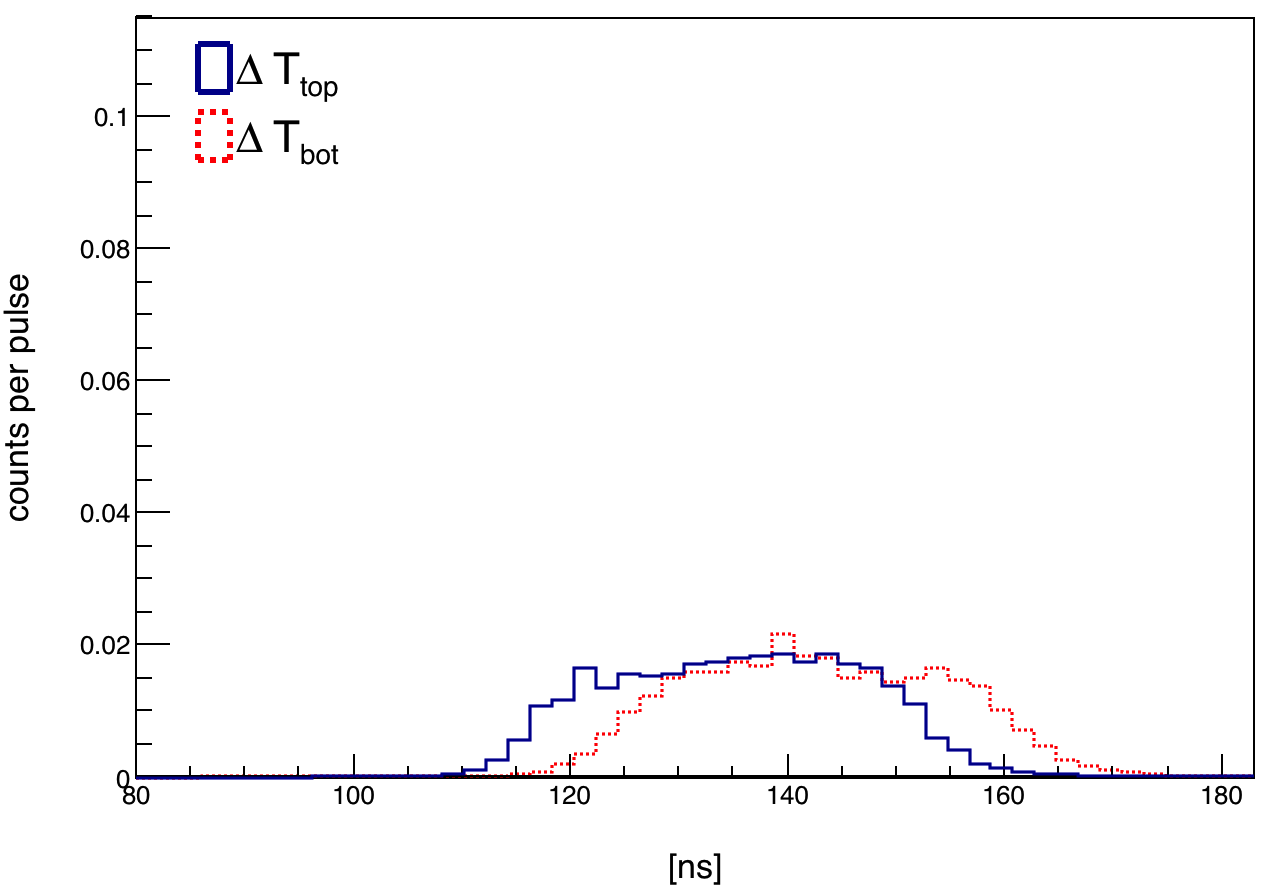
\includegraphics[width=0.5\textwidth]{Content/Methods/ToF0.png}}
\end{center}

\subfloat[$\Delta T$s with Aluminum target.]{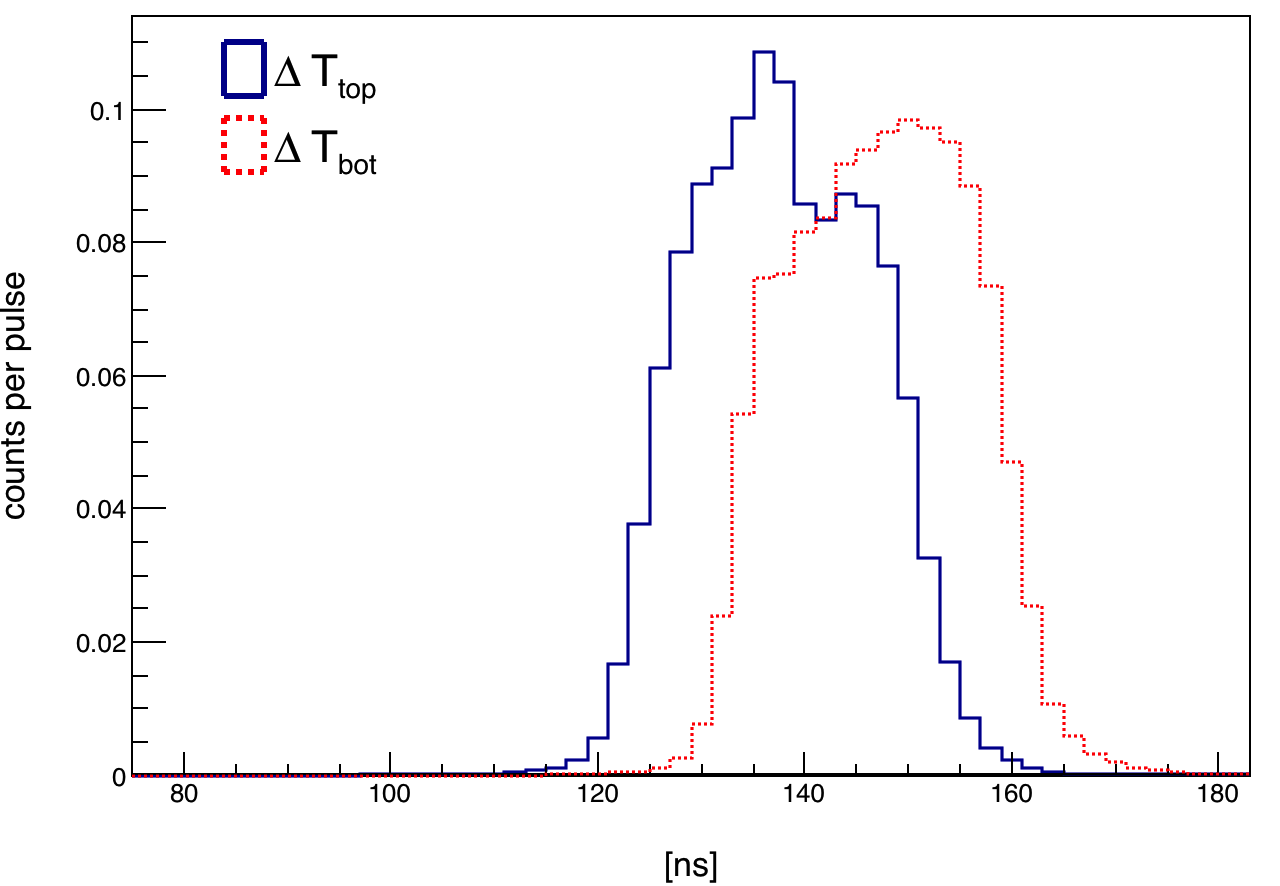
\includegraphics[width=0.5\textwidth]{Content/Methods/ToF1.png}}
\subfloat[Average of $\Delta T_{\text{top}}$ and $\Delta t_{\text{bot}}$  with Aluminum target in place.]{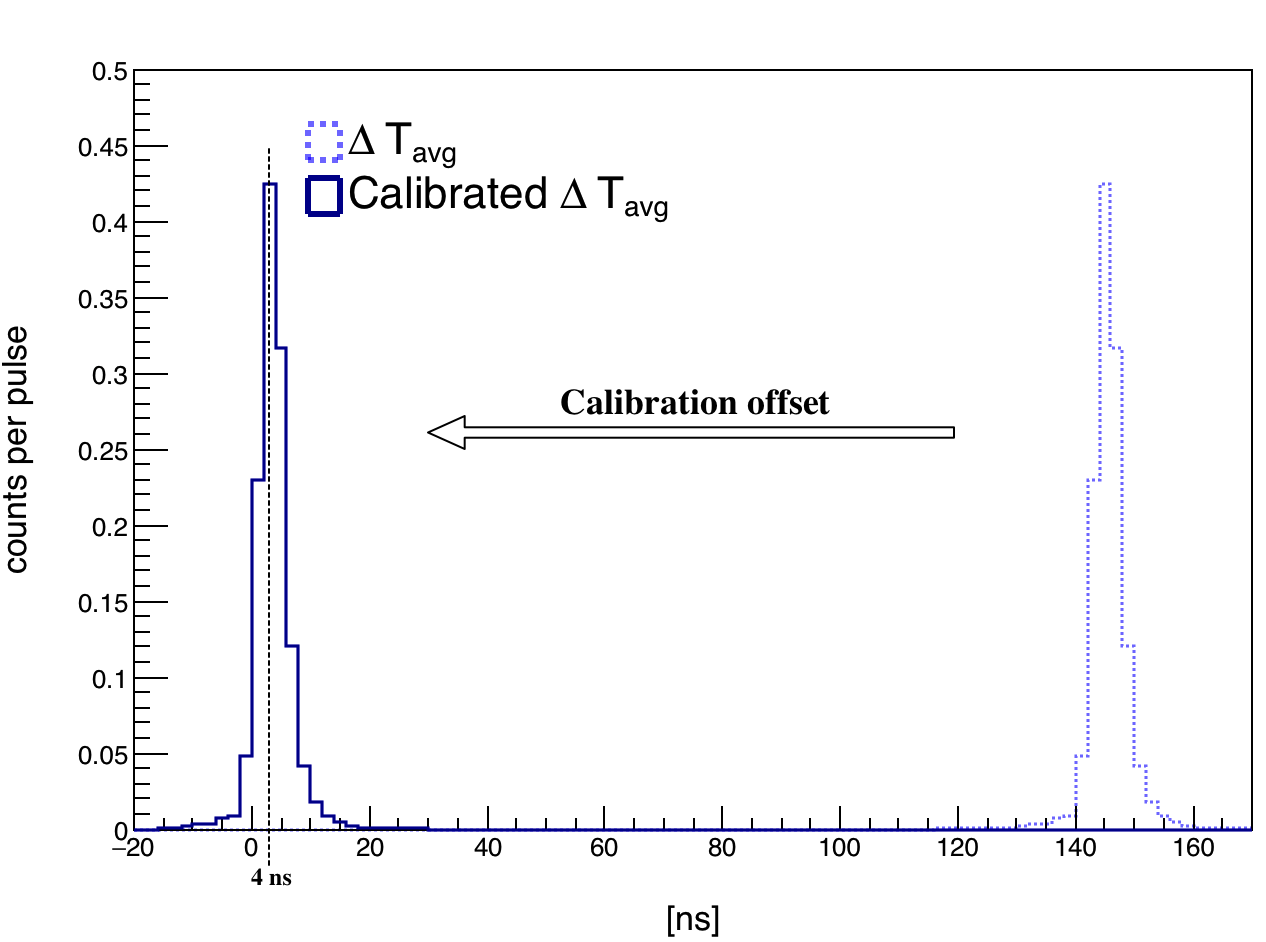
\includegraphics[width = 0.5\textwidth]{Content/Methods/ToF2.png}}
\caption{(a) $\Delta T$ spectra from each PMT of a detector with no target in place.
The beam dump is not able to collect all excess photons, so there is a background despite the lack of a target to scatter photons into the detectors.
The background is caused by photons that scatter from various surfaces within the experimental cell.
(b) The introduction of a non-neutron producing target made from aluminum produces a peak caused by the scattering of photons from the target.
These photons have a constant time of flight, so the width of these spectra are reflective of the range of times taken for scintillation light to propagate from the points of scintillation to a PMT.
(c) Taking the average between the $\Delta T$s of the top and bottom PMT gives a sharper peak, since the sum of times from both PMTs is a reflection of the time required for light to travel the entire length of a detector, regardless of the location of the particle hit.
The correct timing offset can be now be found since the photons have a time of flight of 4 ns. }
\label{fig:ToFDetermination}
\end{figure}
   
\subsection{Particle Position Reconstruction}
% ToDo: The determionation of position could use a figure. The figure could indicate verticle reconstruction, and horizontal error. 
Spacial resolution in the horizontal plane is determined by the physical dimensions of the detector.
The geometric center of a detector is used for the position, in the horizontal plane, of a particle hit.
The detector's dimensions in the horizontal plane are comparatively small at 3.8x15 cm$^2$, so in doing this, a positional uncertainty of $\pm$7.5 cm is introduced, which expressed in terms of an angle is $\pm4^{\circ}$.
The final results of this work use an opening angle bin width of 20$^{\circ}$, so $\pm4^{\circ}$ is not large enough be a cause for concern.
The largest contributor to uncertainty in particle position is the position in the vertical direction, which is determined by the timing difference between signals in the top and bottom PMTs.

The determination of a particle's position in the vertical direction relies on the timing of coincident signals from both the PMTs of a detector.
The timing difference obeys a linear relationship with respect to the location of the particle hit along the length of the detector.
The z-coordinate will hereafter refer to a particle's position along the vertical axis, where $z=0$ corresponds to the geometric center of the detectors.

As discussed before, detected scintillation light tends to take fairly direct paths to the PMTs, experiencing few reflections off the boundary of the scintillation cell.
As a result, the timing difference between signals in the top and bottom PMTs is proportional to the difference in path lengths that the scintillation light must travel to reach each PMT, which is in turn proportional to the z-coordinate of the particle hit.
The exact linear relationship is determined through calibration by using collimated photons from a $^{60}$Co source.
Calibration is achieved by measuring the PMT top-bottom timing difference while the $^{60}$Co source is fixed at five different locations along the detectors length.
The setup for calibration was discussed in section~\ref{reconstruction}.
The result is shown in figure~\ref{fig:PMTDifference}.

\begin{figure}
    \centering
    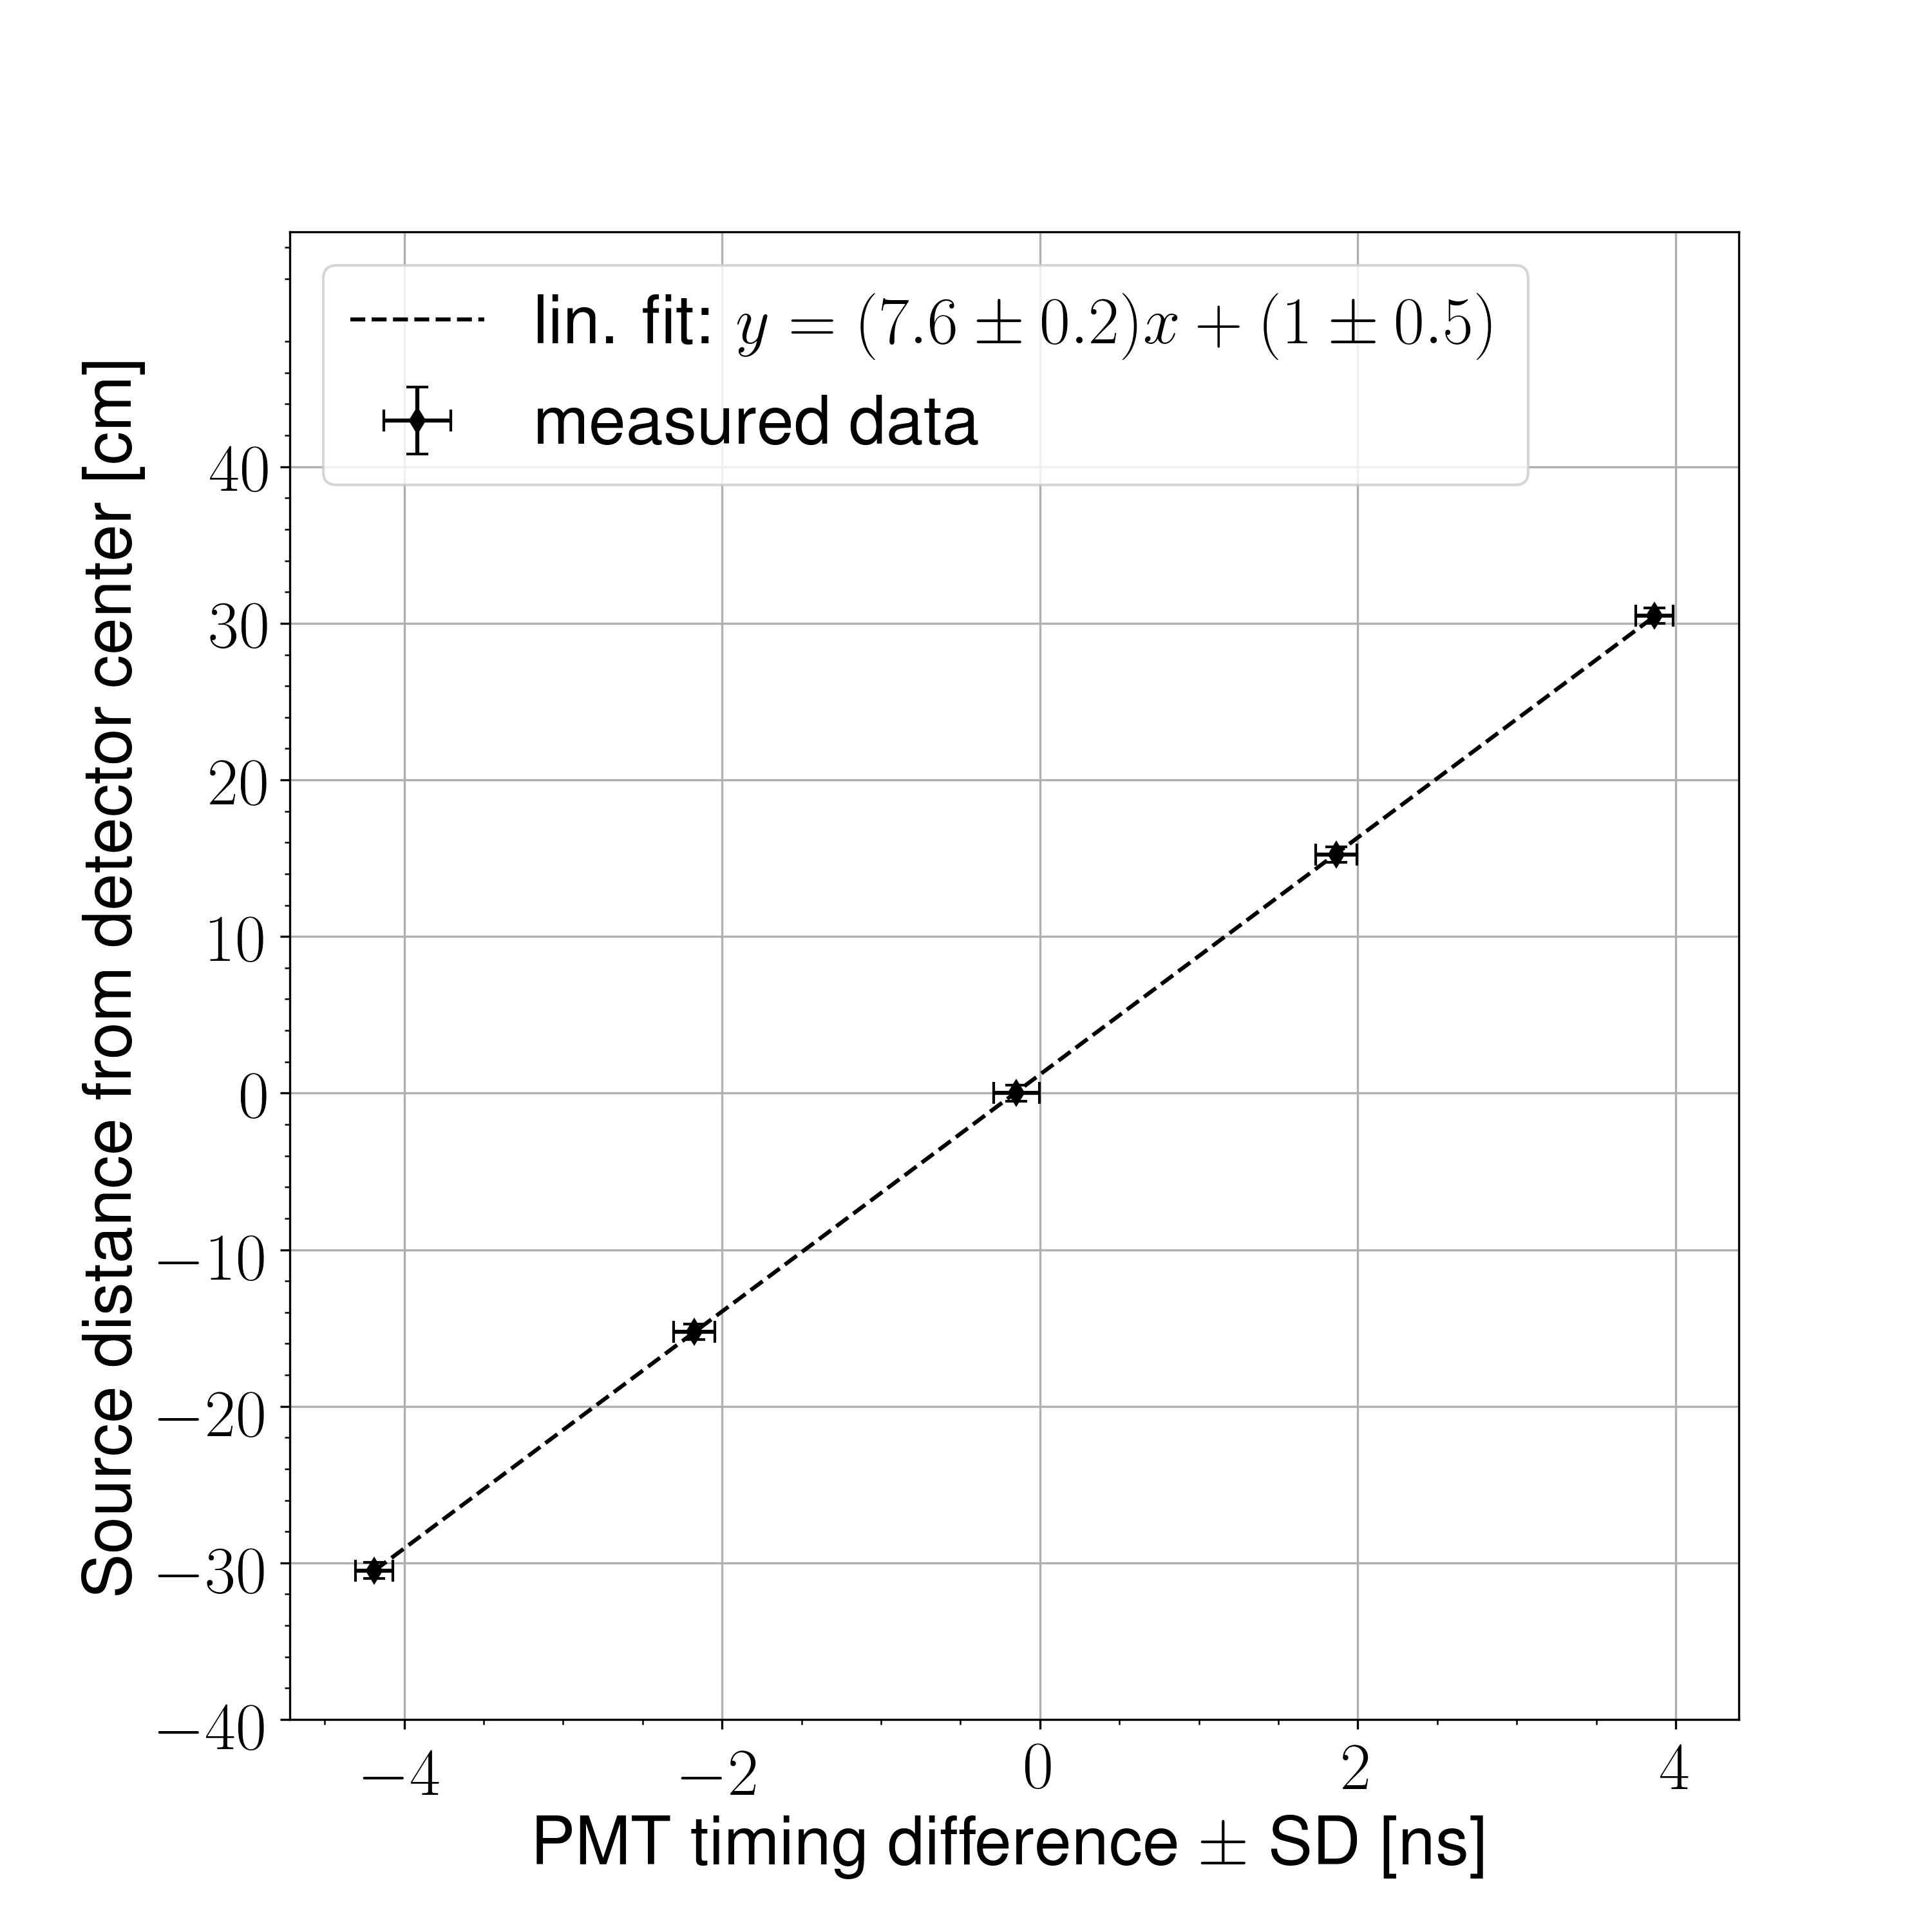
\includegraphics[width = 0.9\textwidth]{Content/Methods/PMTDifference.png}
    \caption{A collimated $^{60}$Co source is used to produce events at precise locations on the detector.
    The particle's position along the detector's length is shown to vary linearly with respect to the timing difference between events in the top and bottom PMTs of a detector.}
    \label{fig:PMTDifference}
\end{figure}
\subsubsection{Detector Shielding}
The detector's shielding was designed with the aim of reducing cross-talk, the detection of photons, and noise.
The front face of the detectors, facing towards the target, were subject to the highest gammas flux due to the scatting of the beam from the target.
The detection of a gamma renders a detector ``dead'' during the time at which subsequent fission neutrons from the same pulse reach the detector.
Lead can mitigate this problem by attenuating gammas, but has the side effect of scattering neutrons.
If a neutron scatters prior to being detected, the ToF calculation will be incorrect because the neutron traveled an unknown distance to the detector.
The extent that neutron distances of travel are perturbed due to scattering from lead shielding was quantified using an MCNP .
% ToDo: Add figure of neutron position variance cause by lead scattering.
Accordingly, 1" of lead was placed along the front face of the detectors.
%ToDo: use actual gama rate in the sentance below once the wiki is back up.
This diminished gamma detection rates to reasonable levels and, according to the simulation, caused a negligible amount of neutron scattering.
Because of particularly high gamma flux, an additional 2" of lead was placed at the sides of detectors adjacent to the beam, and along the front faces of the detectors farthest downstream at $\pm30^{circ}$ from the beam line.
Placing lead behind the detectors was avoided in consideration of an MCNP-POLIMI simulation, which indicated that lead placed here facilitates cross-talk.
Because cross-talk events are in fact correlated, they cannot be removed in analysis by the subtraction of accidentals.
For more information about cross-talk, see section~\ref{crosstalk}.

\subsection{Targets}
\todo{Pictues of target}
A depleted uranium (DU) target with dimensions of 4x2x0.05 $\text{cm}^3$ was used as the primary target for the measurement of two-neutron correlations.
DU received the majority of the allotted beam time because it is an even-even nucleus and as a consequence the fission fragments are emitted with a high degree of anisotropy~\cite{1977FragAss}.

It is desirable to have a target geometry with symmetry that is consistent with the cylindrical symmetry of the neutron detector array.
To accomplish this, a thin rectangular target was rotated slowly about the vertical axis during data acquisition.
In doing so, the measurement is reflective of the average of events which occurred while the target was at all orientations between 0 and 2$\pi$, thereby cylindrical symmetry is effectively preserved.
This eliminates potential biases caused by the asymmetrical structure of the target.

\subsection{Measurements with $^{252}$Cf}
%ToDo: Place our results of Cf measurements here in comparison to past measurements.

Opening angle measurements were also performed on neutrons from the spontaneous fission (SF) of $^{252}$Cf.
There is good agreement among past measurements of the opening angle distribution of neutrons from the spontaneous fission of $^{252}$Cf, and so such measurements serve as a means to validate the methods used in this study.

As opposed to the measurements of neutrons from photofission, there is no concern over the detection of accidental neutron pairs, because given the strength of the $^{252}$Cf source, it is highly unlikely that two fissions occur during the acceptance time window of 150 ns.
Another difference between the two measurements is the clean and sharp peak produced by fission photons from $^{252}$Cf, compared to a relatively smeared peak produced by photons scattering from the target during measurements of photo-neutrons.
In each measurement, the photon peak is used as a reference point for the calculation of neutron ToF.
As a result the $^{252}$Cf measurements have less error in ToF caused by the spreading of the photon peak used for reference.
The same normalization technique is used for both measurements, in which the correlated distribution is divided by the uncorrelated distribution of neutron pairs taken from different fissions.

The configuration for this was different than that for photofission measurements, as the photon beam can no longer be used for the timing of a ``start'' trigger.
The trigger for $^{252}$Cf consisted of two high timing-resolution scintillation photon detectors made from ATP plastic, where one is fixed below and the other above the source at a distance of 15 cm.
Using a coincidence window of 4 ns, the timing start trigger required 2-fold coincidence between both the photon detectors.
Aside from a different mechanism for a start trigger, the methods used for the measurement of two-neutron opening angle distributions in the SF of $^{252}$Cf are equivalent to those used for photofission.


